\subsubsection{Dimensionnement}

Pour supprimer la composante continue, il suffit d'ajouter un filtre passe-haut. Nous n'avons aucune contrainte sur ce filtre, à part le fait qu'on ne doit évidemment pas atténuer les fréquences utiles. C'est pourquoi on a choisi un filtre dont la fréquence de coupure est de 90 Hz\footnote{La plus petite fréquence utile est de 900 Hz et la règle de bonne pratique est de prendre une fréquence de coupure dix fois plus petite que cette fréquence}. 

Pour dimensionner ce filtre (et le filtre de Butterworth), nous utilisons le site internet suivant : \url{https://tools.analog.com/en/filterwizard/}. 

Nous obtenons le filtre suivant sur la Figure \ref{fig:highpass}, les détails des paramètres sont disponibles dans l'annexe \ref{hfilterannexe} :

\begin{figure}[H]
    \centering
    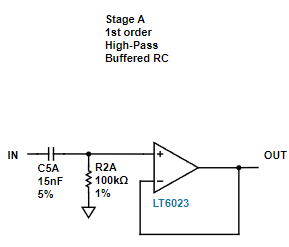
\includegraphics[width=0.4\textwidth]{Pictures/highpassfilter.png}
    \caption{Filtre passe-haut}
    \label{fig:highpass}
\end{figure}

Ce filtre est suivi d'un buffer. A partir de ce dernier, on peut déjà construire  un premier étage amplificateur. Mais avant, il nécessaire de polariser le signal car les ampli-op ont une plage de fonctionnement allant de 0V à 3.3V.

La polarisation va dépendre du type d'amplification que nous allons réaliser. Nous avons le choix entre deux types : \textbf{Amplificateur non-inverseur} ou \textbf{Amplificateur inverseur}. Le tableau \ref{tab:tabamp} reprend les caractéristiques des méthodes.

\begin{table}[H]
    \centering
    \begin{tabular}{|c|c|c|}
    \hline
        \cellcolor[RGB]{100,100,100}&\textbf{Non-inverseur} & \textbf{Inverseur} \\
        \hline
         \textbf{Gain} & $1+\frac{R_1}{R_2}$ & $-\frac{R_1}{R_2}$\\ 
         \hline
         \textbf{Impédance d'entrée} &  $\infty$& $R_2$\\
         \hline
         \textbf{Choix des résistances pour le gain} & Indépendant du filtre & Dépendant du filtre \\
         \hline
    \end{tabular}
    \caption{Tableau comparant l'amplificateur non-inverseur et inverseur}
    \label{tab:tabamp}
\end{table}

Nous allons opter pour un amplificateur non-inverseur car le gain que nous devons atteindre est très grand (plus de $60$dB) et nous avons préféré avoir la plus grande flexibilité possible dans le choix des résistances responsables de l'amplification.

La polarisation de ce type de montage se réalise en ajoutant un diviseur résistif à la borne positive de l'ampli-op. La valeur des résistances doivent être identique pour avoir une polarisation autour de $1.65\ V$ :

\begin{align*}
    1.65 &= 3.3 \ V \times \frac{R_2}{R_1+R_2}\\
    \iff R_1&=R_2
\end{align*}

On pourrait se dire que la valeur de la résistance doit être de $100 \ k \Omega$ comme indiqué dans la figure \ref{fig:highpass}. Si on fait cela, la fréquence de coupure du filtre passe-haut est décalée vers la droite car ces deux résistances sont en parallèle. Ainsi, c'est la résistance équivalente des résistances de polarisation qui doit valoir $100 \ k \Omega$ :

\begin{align*}
    R_{eq}&= \frac{R_1 \ R_2}{R_1 + R_2 }\\
    \iff 100 \ k \Omega&= \frac{R}{2}\\
    \iff R&=200 \ k \Omega
\end{align*}

Cependant, dans la série E12, il n'y a pas de résistance de $200 \ k \Omega$. On va utiliser la résistance supérieure la plus proche et elle vaut $220 \ k \Omega$. 

Le décalage de la fréquence de coupure est visible sur la courbe de Bode\footnote{Le circuit de simulation LTspice est disponible dans l'Annexe \ref{ltspiceHighPassResistors} } de la figure \ref{fig:bodehighpasspol}

\begin{figure}[H]
    \centering
    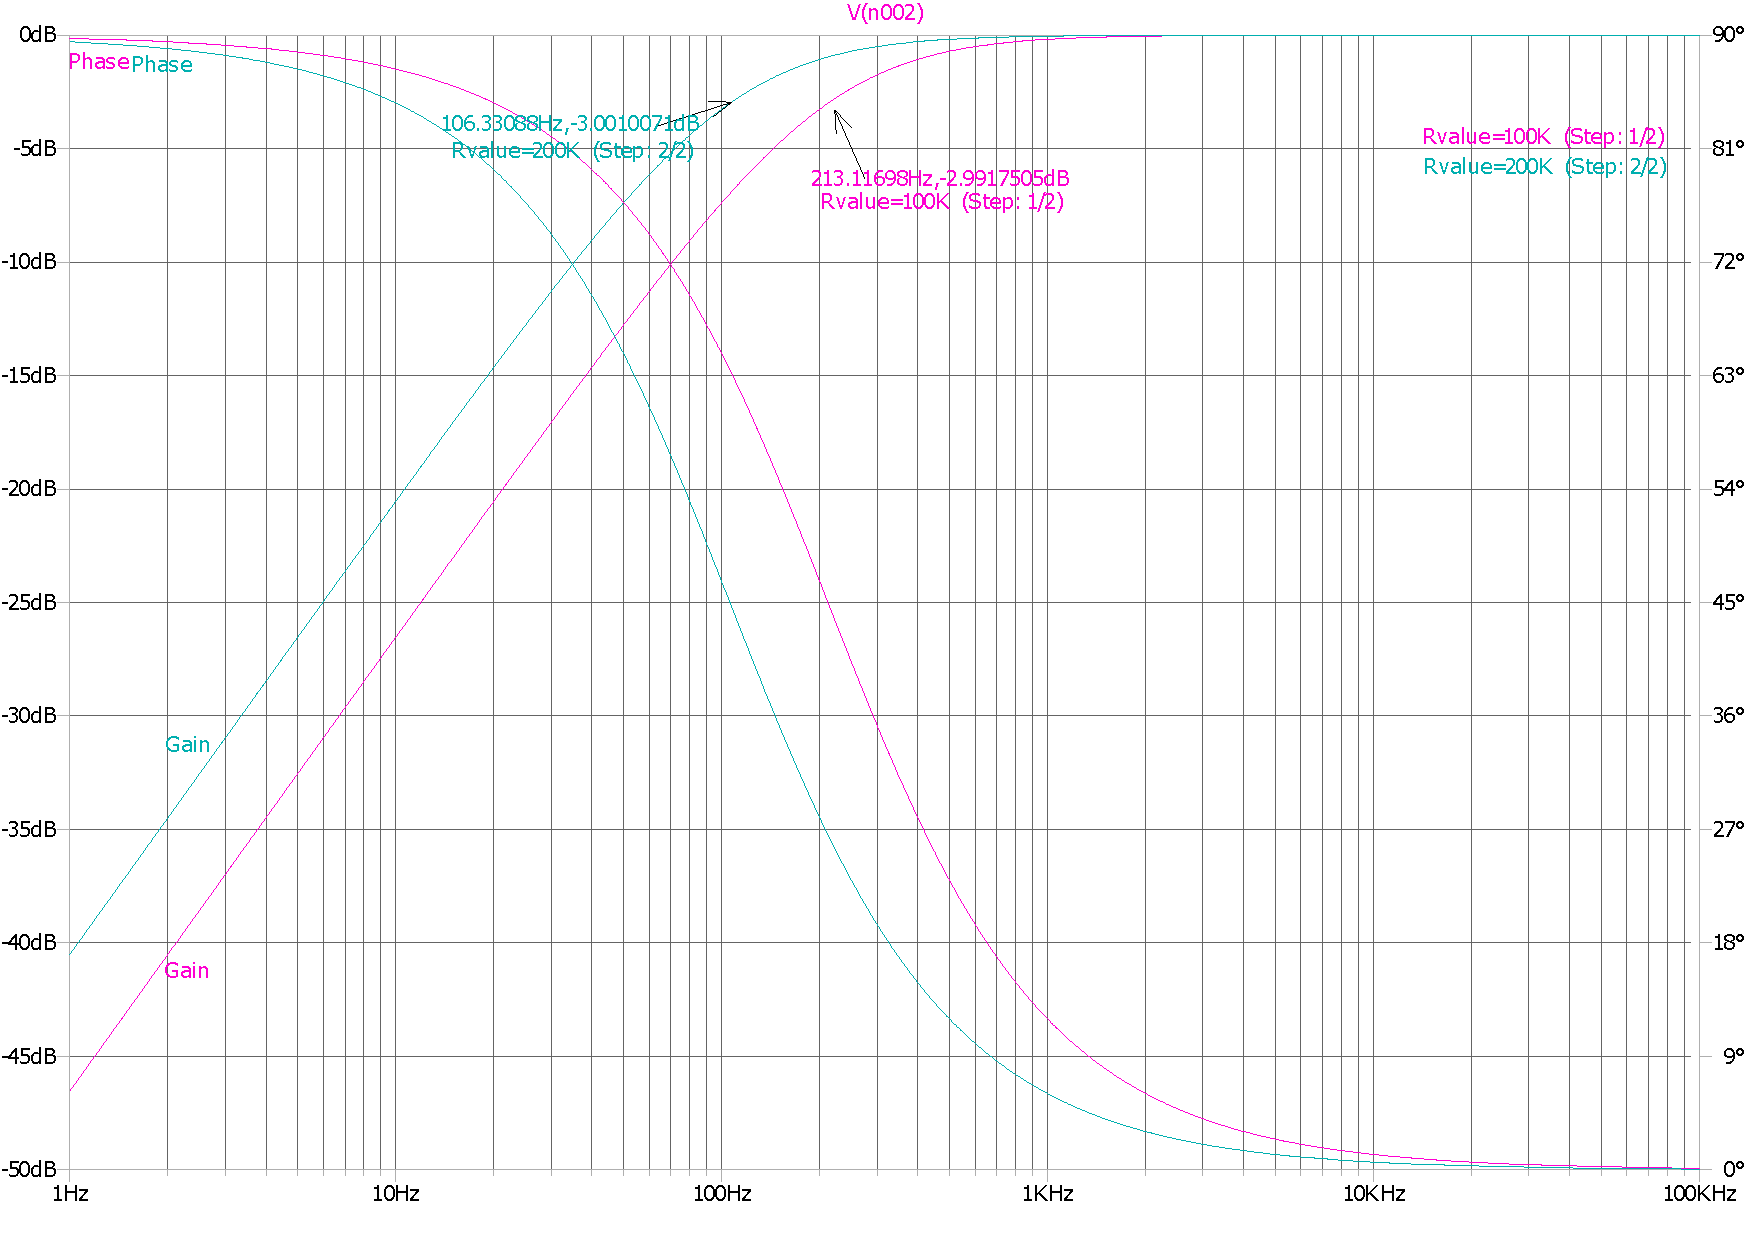
\includegraphics[width=\textwidth]{pdffiles/HighPass/BodeHighPassPolarization.pdf}
    \caption{Courbe de Bode du filtre passe-haut avec un diviseur résistif. $100 \ k \Omega $ en rose et $200 \ k \Omega$ en bleu}
    \label{fig:bodehighpasspol}
\end{figure}


La Figure \ref{fig:poldiag} représente le bloc \textbf{Amplification} après suppression de la composante continue et polarisation du signal.

\begin{figure}[H]
    \centering
    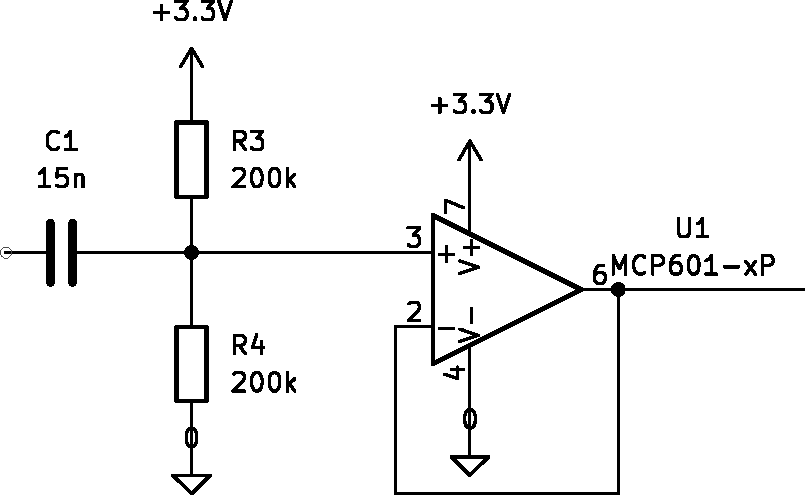
\includegraphics[width=0.5\textwidth]{pdffiles/poldiag.pdf}
    \caption{Filtre passe-haut avec polarisation}
    \label{fig:poldiag}
\end{figure}

Il ne reste plus qu'à amplifier le signal. Avant de rajouter les résistances, il faut qu'on détermine le nombre d'étage nécessaire pour obtenir le gain voulu à l'aide du produit \textbf{Gain x Bande passante}.

Le laboratoire nous fournit des ampli-op \textbf{MCP601}. Le \textbf{GBWP} de ce dernier, disponible dans la datasheet (voir annexe \ref{datasheet}), vaut $2.8 \ MHz$. Sachant que la plus haute fréquence utilisée vaut $1.1 \ kHz$, on a :

\begin{align*} 
 & \text{Gain} \times 1100 = 2.8 \times 10^{6} \\ 
\iff & \text{Gain} = \frac{2.8 \times 10^{6}}{1100}=2545.454545=68.11530 \ dB
\end{align*}

Le gain maximal d'un seul étage dans la bande passante qui nous intéresse vaut environ 2545, ce qui est au-dessus du gain  qu'on voulait obtenir. On peut donc amplifier notre signal avec un seul ampli-op. Il n'est donc pas nécessaire d'ajouter de gain dans le filtre de garde.

Pour le choix des résistances, on peut calculer le rapport entre $R_1$ et $R_2$ :

\begin{align*}
    1+ \frac{R_1}{R_2} &= 1650 \\
    \iff \frac{R_1}{R_2} &= 1649
\end{align*}

Il faut fixer la valeur de $R_2$ pour trouver celle de $R_1$. Il y a trois choses à prendre en compte :

\begin{itemize}
    \item [$\bullet$] La résistance $R_2$ ne doit pas être trop grande (en dessous de 10k)
    \item [$\bullet$] On doit utiliser les résistances à notre disposition (la série E12)
    \item [$\bullet$] La résistance $R_2$ doit faire en sorte que son rapport avec la capacité de sortie soit le même que celui du filtre en amont.
\end{itemize}

Le dernier point concerne l'ajout d'une capacité à la sortie de l'ampli-op. En effet, si on ajoute des résistances pour le gain, la polarisation ne sera plus la même car il y a aura une chute de potentiel. On doit rajouter une capacité à la sortie de l'étage pour conserver cette polarisation. Le rapport entre la résistance $R_2$ et la capacité de sortie doit être la même que le rapport du filtre à l'entrée\footnote{Pour ne pas atténuer les fréquences utiles}. Le tableau \ref{tab:tabres} reprend les valeurs que nous avons choisies avec une brève justification.

\begin{table}[H]
    \centering
    \begin{tabular}{|c|c|l|}
    \hline
        \cellcolor[RGB]{100,100,100}&\textbf{Valeur} & \textbf{Justification} \\
        \hline
         \textbf{$R_1$} & $2.473520 \ M \Omega$ & Normalement il faudrait $2.473500 \ M \Omega$  mais la valeur choisie reste très proche.\\ 
         && On l'obtient en mettant en série les résistances suivantes : \\
         && $2.2 \ M\Omega$ ; $270 \ k\Omega$ ; $3.3 \ k\Omega$ ; $220 \ \Omega$ \\ 
         \hline
         \textbf{$R_2$} & $1.5 \ k \Omega$ & Pour avoir une résistance $R_1$ réalisable à l'aide de la série E12, 
          \\ &&$R_2$ doit valoir $1.5 \  X \Omega$. L'ordre de grandeur X est déterminé 
           \\ &&par la capacité de sortie car on ne peut pas avoir une capacité trop grande  \\
         \hline
         \textbf{$C_{sortie}$} & $1 \mu F$ & Pour avoir une résistance $R_1$ dans un ordre de grandeur plus petit que 10k, 
         \\ && il faut choisir une capacité entre $1 \ \mu F$\ et $10 \ \mu F$.\ \\
         \hline
    \end{tabular}
    \caption{Tableau comparant l'amplificateur non-inverseur et inverseur}
    \label{tab:tabres}
\end{table}

Finalement le bloc \textbf{Amplification} est repris sur la figure \ref{fig:blocampli} après avoir rajouté le gain :

\begin{figure}[H]
    \centering
    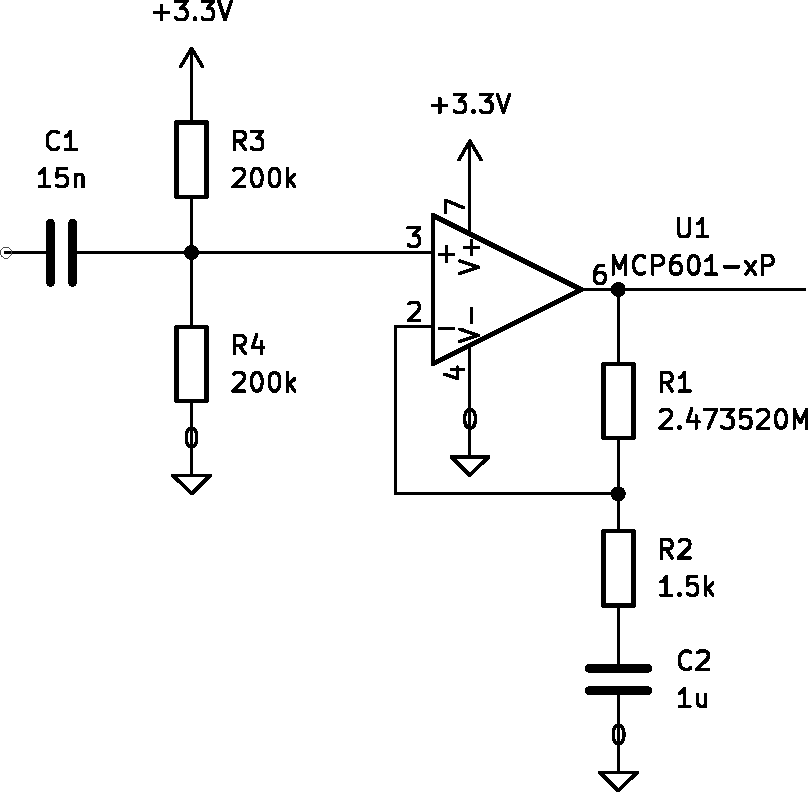
\includegraphics[width=0.5\textwidth]{pdffiles/blocampli.pdf}
    \caption{Bloc Amplification}
    \label{fig:blocampli}
\end{figure}

\subsubsection{Validation du bloc}

Après avoir dimensionné le bloc \textbf{Amplification}, il faut le tester pour valider son fonctionnement. Pour cela, il suffit d'ajouter le microphone en entrée et de mesurer à l'aide d'un Picoscope la sortie de cet étage. Le signal de sortie doit avoir l'allure suivante : un signal sinusoïdal variant de $0 \ V$ à $3.3 \ V$, centré en $1.65 \ V$.